\subsubsection{Vorticity distribution}
To better understand the distribution of vorticity generation within
the gas-liquid mixture region of the interface we perform an order of
magnitude analysis to compare the baroclinic vorticity from equation
\eqref{eq:baroclinic_vorticity} in pure water vs air. As this can
already be evaluated in water from what we have provided up to this
point, we will focus on evaluation of the order of baroclinic
vorticity generation in air.

Throughout this analysis we will denote the properties of the incoming
wave and water with a subscript $-$, and the transmitted wave and air
with a subscript $+$. For water, we will use the values for
$\Delta \rho_I, \Delta L_I, \Delta \rho_a, \Delta L_a$ and $\theta$
previously defined in the section \ref{subsubsec:oom_analysis}, based
on our initial condition. Our treatment of the density gradient across
the interface will remain unchanged for evaluation in air such that
$\Delta \rho_I^-=\Delta \rho_I^+$ and $\Delta L_I^-=\Delta L_I^+$. To
evaluate the remaining terms in air we will borrow techniques from
linear acoustics. To find the pressure rise in the transmitted wave
$\Delta p_a^+$, we recognize that $a_0/\ell<<1$ and treat the
incoming wave as a plane wave impinging normally on a flat material
interface such that $\Delta p_a^+=\bs{T} \Delta p_a^-$, where $\bs{T}$
is the acoustic transmission coefficient,
$\bs{T}=2\rho^+ c^+/\left(\rho^+ c^+ + \rho^- c^- \right)$
\citep{Kinsler1982}. For our water-air interface
$\bs{T}\approx4.97\times10^{-4}$. Because of the strong impedance
mismatch between fluids, the acoustic wave is almost entirely
reflected, decreasing the pressure gradient in the air. Because of the
drop in sound speed across the interface, the transmitted wave is
compressed into a smaller physical area (i.e., the wavelength
decreases) relative to the incoming wave, such that
$\Delta L_a^+=\Delta L_a^- (c^+/c^-)$. This effect increases the
pressure gradient in the air. To evaluate $\theta^+$, we utilize
Snell's law which states that
$c^-\sin{\theta^-}=c^+\sin{\theta^+}$. Because $a_0/\ell<<1$ it is
also true that $\theta^-<<1$, thus we use the small angle
approximation of $\sin$ to find that
$\theta^+\approx\theta^-(c^+/c^-)$. This refraction effect decreases
the misalignment between the pressure and density gradients for the
transmitted wave relative to the incoming wave. Quantitatively it also
approximately cancels the increase in vorticity deposition that arises
as a result of the increased pressure gradient created by the decrease
in the length of the transmitted wave.

To get an idea of where within the mixed gas-liquid region at the
interface the vorticity will be generated, we consider equation
\eqref{eq:baroclinic_vorticity} in air and water and write the ratio
to find
\begin{align}%
  \label{eq:baroclinic_air_water}%
  % \left(\frac{\partial\omega}{\partial t}\right)_{\substack{\text{baroclinic}\\\text{air}}} / \left(\frac{\partial\omega}{\partial t}\right)_{\substack{\text{baroclinic}\\\text{water}}}%
  \frac{\norm{\frac{\nabla\rho\times\nabla p}{\rho^2}}_{air\quad}}{\norm{\frac{\nabla\rho\times\nabla p}{\rho^2}}_{water}}
  =&\orderof{\frac{\left[\frac{\abs{\Delta \rho_I^+}}{\abs{\Delta L_I^+}}\frac{\abs{\Delta p_a^+}}{\abs{\Delta L_a^+}}\frac{1}{\abs{\rho^+}^2}\abs{\theta^+}\right]}
     {\left[\frac{\abs{\Delta \rho_I^+}}{\abs{\Delta L_I^+}}\frac{\left(\abs{\Delta p_a^+}/\abs{\bs{T}}\right)}{\abs{\Delta L_a^+}\left(\abs{c^+}/\abs{c^-}\right)}\frac{1}{\abs{\rho^-}^2}\left(\abs{c^+}/\abs{c^-}\right)\abs{\theta^+}\right]}},\nonumber\\%
  =&\orderof{\abs{\bs{T}}\left(\frac{\abs{\rho^-}}{\abs{\rho^+}}\right)^2}.%
\end{align}
vFor our water-air interface, we evaluate equation
\eqref{eq:baroclinic_air_water} to find that the ratio of baroclinic
vorticity generation in air to that in water would be of order
$\orderof{10^2}$. While this analysis considers vorticity generation
in pure air and water, as opposed to the mixed fluid region that is
exactly relevant to this work, we make two observations based on this
result. First, this result analysis is for an extreme case in which
all of the vortical energy relevant to this problem, is able to be
concentrated in pure air and water, and thus this result acts as an
upper bound on the change in vorticity deposition we expect as the
wave move from water across the interface into air. Additionally, this
result suggests that for the mixed water-air region, where the
strongest density gradient exists, vorticity generation is likely to
occur in gas dominated fluid regions with a higher volume fraction of
air than water.
\begin{figure}[h]
  \centering
  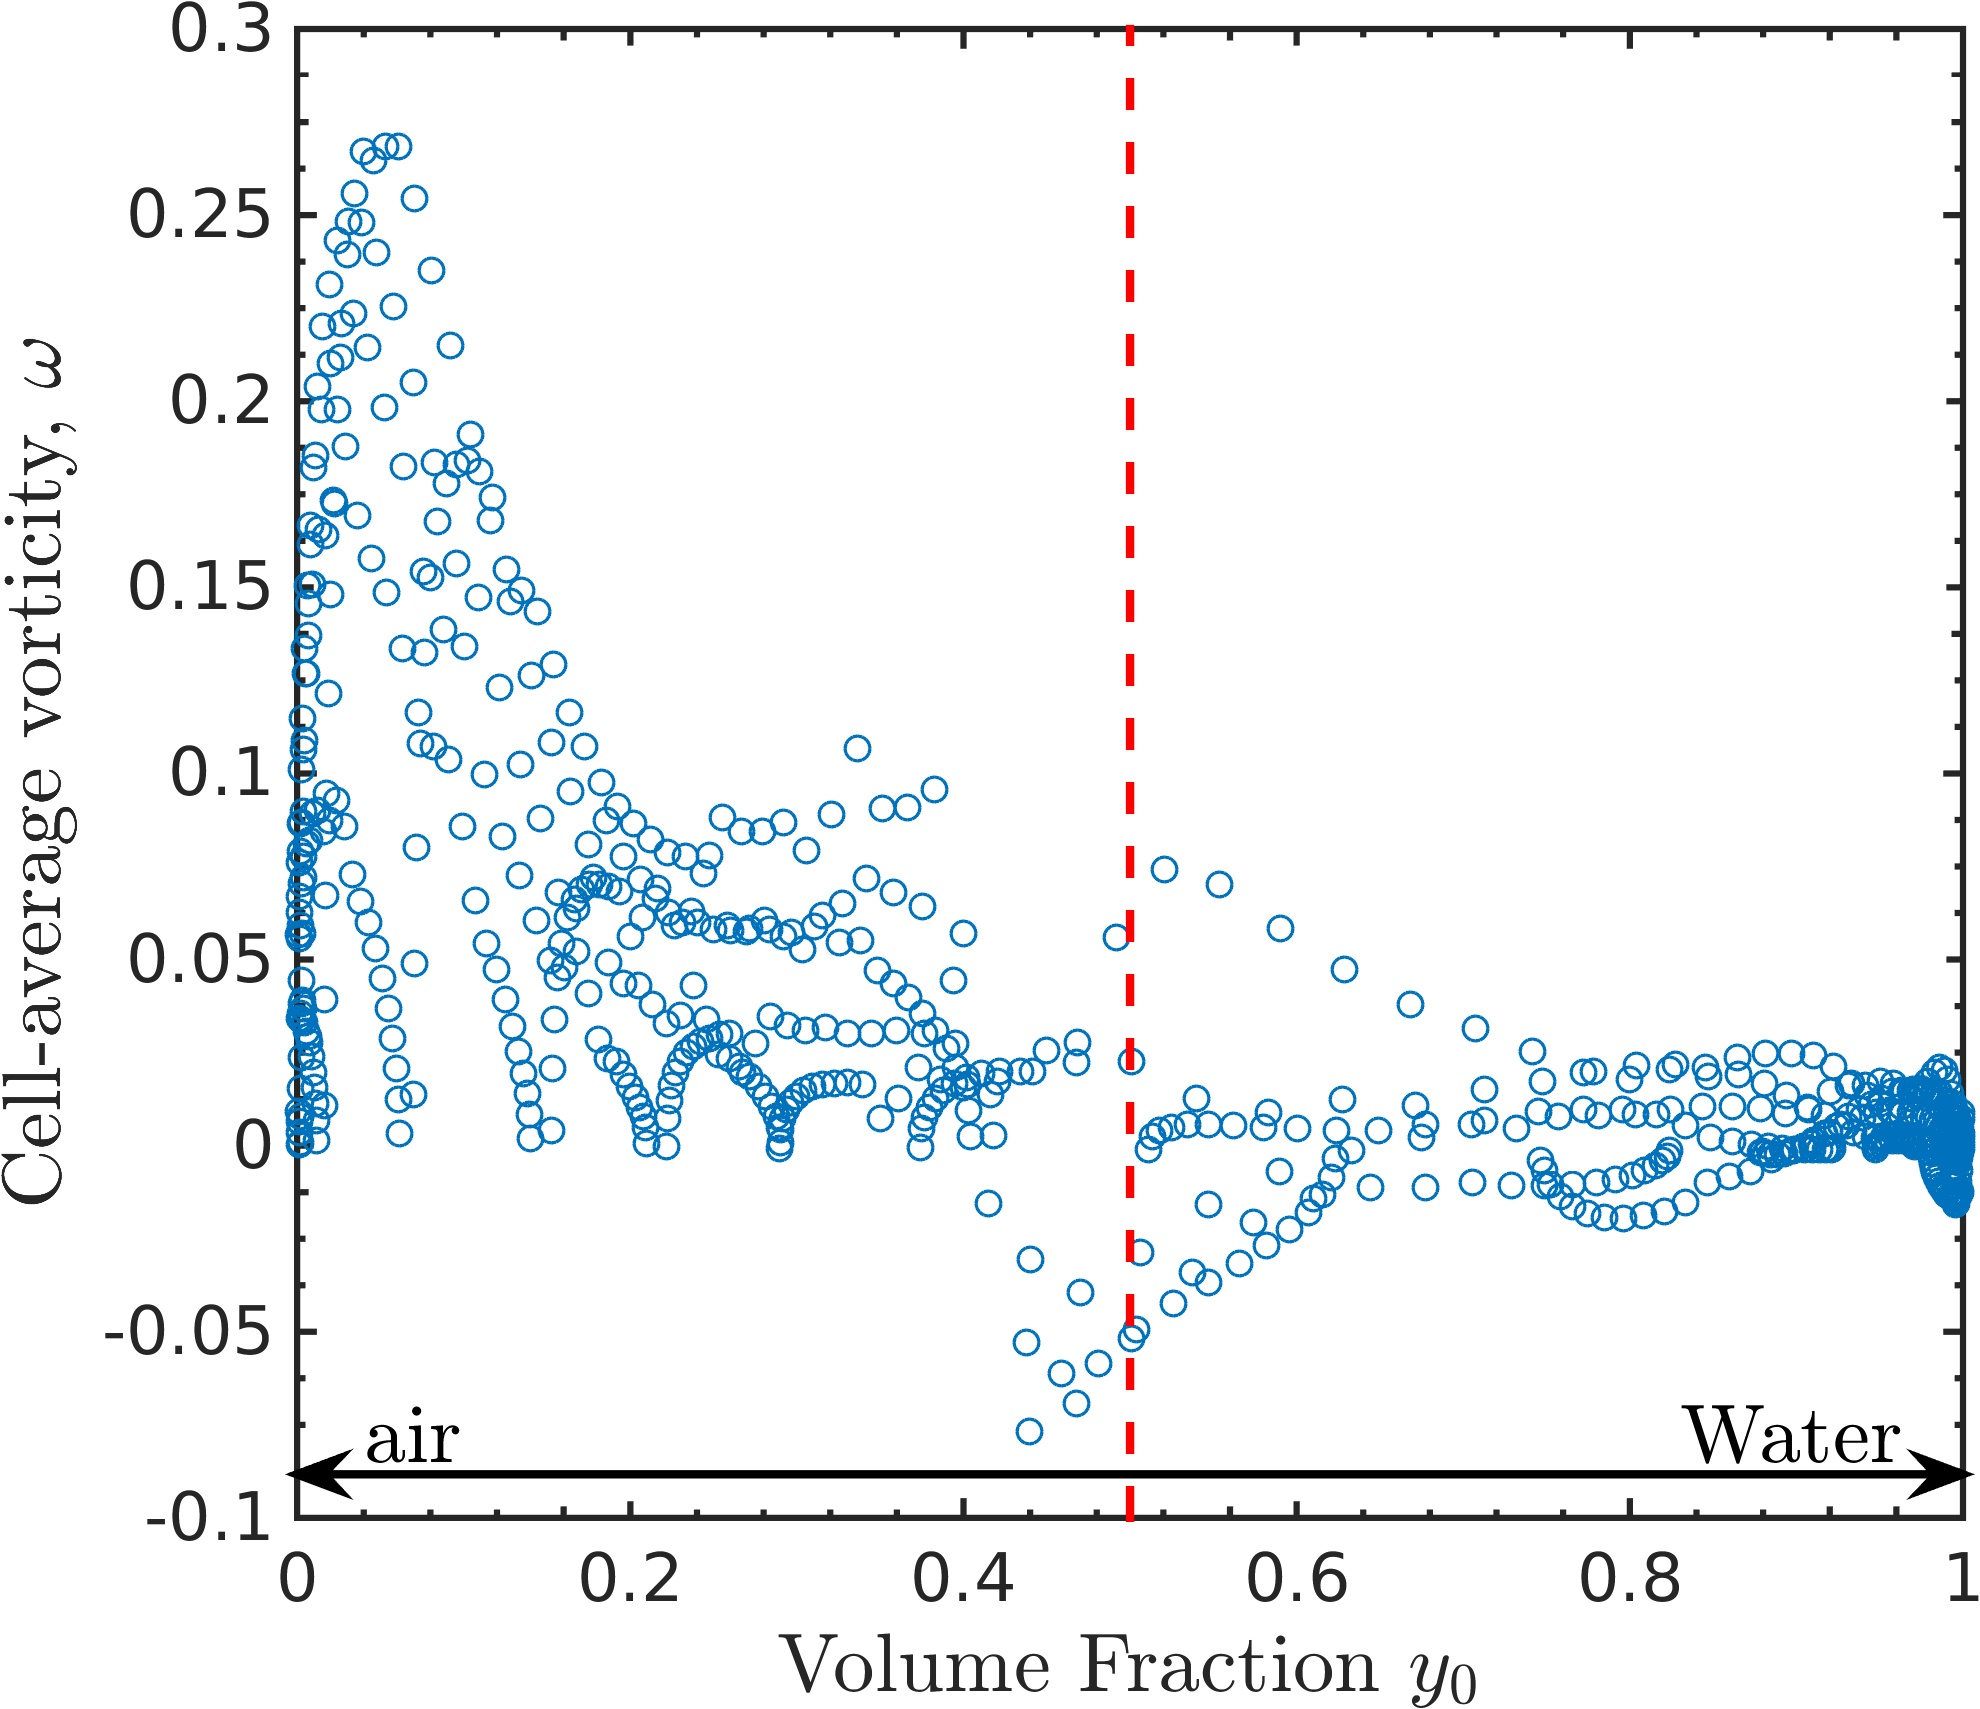
\includegraphics[width=.48\textwidth]{./figs/lung_figs/vorticity_vs_y0} \hfill
  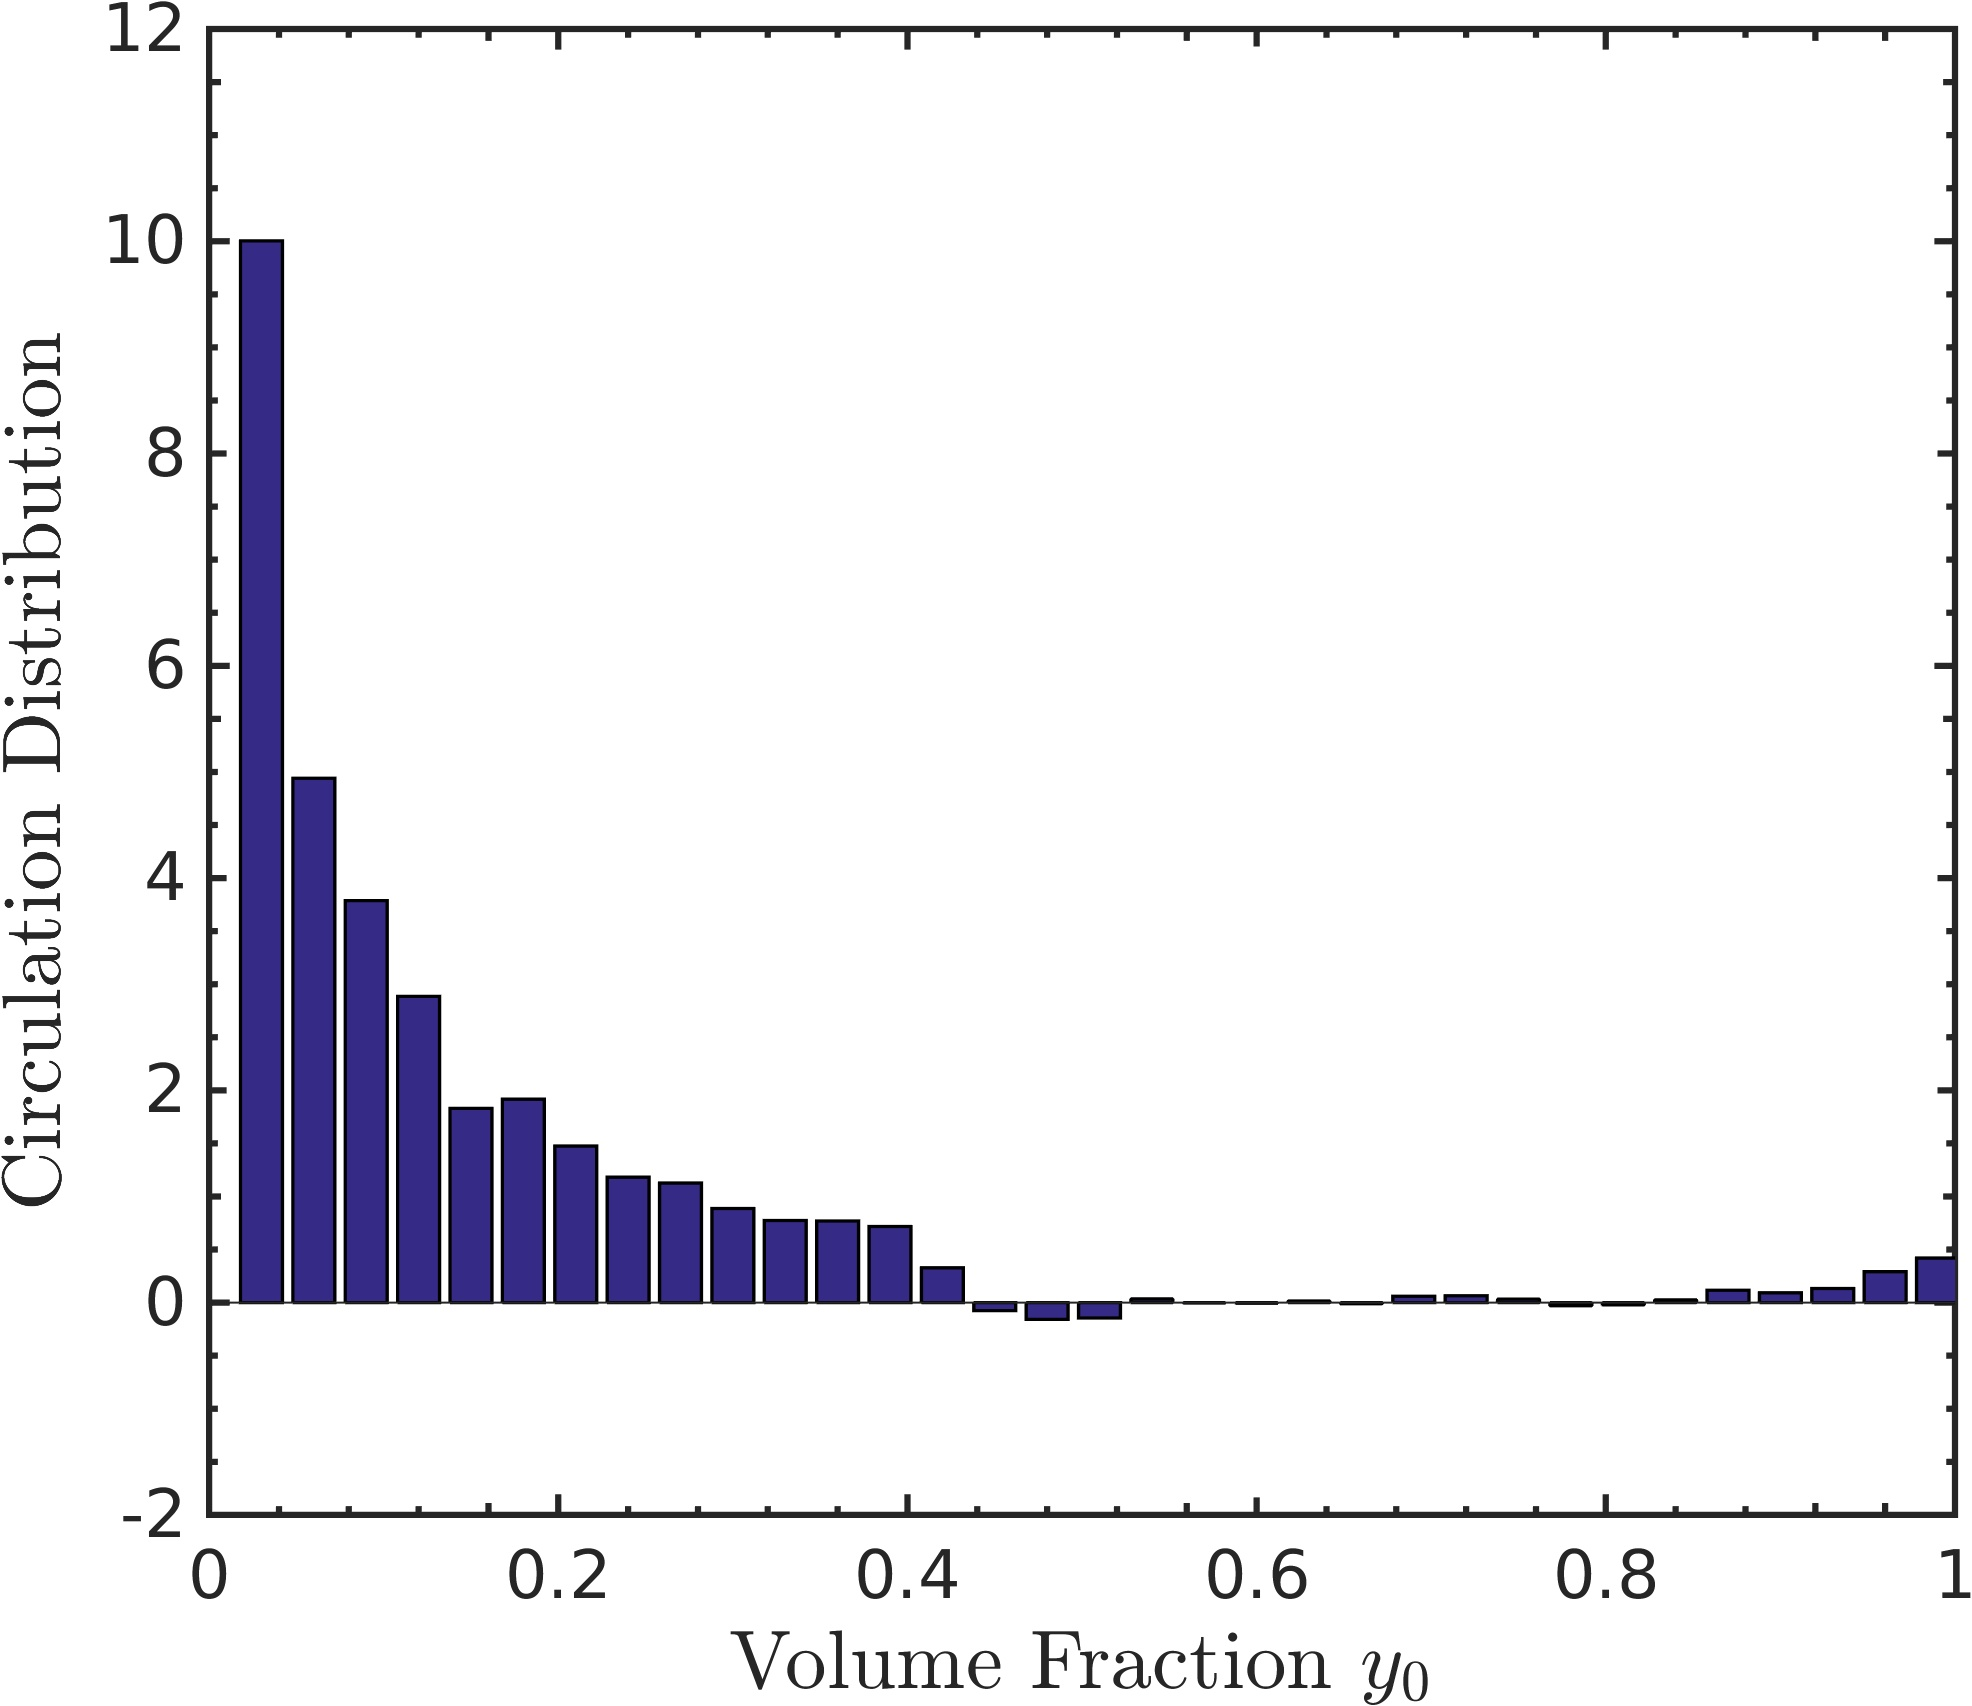
\includegraphics[width=.48\textwidth]{./figs/lung_figs/circ_y0_dist2}
  \caption{For cells with non-negligible vorticity, a scatter plot of the mean vorticity in each cell is plotted as a function of volume fraction water (Left).  }
  \label{fig:baroclinic_y0_distribution}  
\end{figure}

From the vorticity contours at $t=1.0$ shown in
\ref{fig:vorticity_snapshots}, the vorticity is clearly concentrated
in the region with volume fraction of water $\alpha<0.5$. To quantify
this, numerically integrating the vorticity over the right-half domain
we find that 97\% of the circulation occurs in this region. To further
illustrate the dependence of the vorticity deposition on the relative
gas-liquid composition of the fluid within the interface region,
Figure \ref{fig:baroclinic_y0_distribution} shows a scatter plot of
the vorticity values in each cell vs the mean volume fraction of water
in the cell $<\alpha>$ (Left). The average circulation per-cell is
seperated into bins based on the relevant volume fraction to obtain a
histogram and normalized to obtain the circulation distribution
circulation as a function of $\alpha$ (Right). The observed circulation
deposition in air-dominated fluid, $\alpha<0.5$, and is within the
predicted upper bound. This is qualitatively consistent with our
analysis.

%%% Local Variables:
%%% mode: latex
%%% TeX-master: t
%%% End:
